
\documentclass{article}
\usepackage[utf8]{inputenc}
\usepackage[titletoc, title]{appendix}
\usepackage{geometry}
\geometry{
 a4paper,
 left=27mm,
 top=30mm,
 }
\usepackage{ amssymb }
\usepackage{graphicx} % Required for the inclusion of images
\usepackage{caption}
\usepackage{subcaption}
\usepackage{amsmath} % Required for some math elements




\usepackage{hyperref}
\usepackage{float}






%\setlength\parindent{0pt} % Removes all indentation from paragraphs
\usepackage{authblk}
\usepackage{wrapfig}
%\renewcommand{\labelenumi}{\alph{enumi}.} % Make numbering in the enumerate environment by letter rather than number (e.g. section 6)
\usepackage[font={small}]{caption}
%\newcommand*\diff{\mathop{}\!\mathrm{d}}
\usepackage{tikz}
\usepackage{placeins}



%----------------------------------------------------------------------------------------
%	DOCUMENT INFORMATION
%----------------------------------------------------------------------------------------

\title{Simple model(s) of population growth} % Title

\author{Florian \textsc{Leprévost}} % Author name

\date{\today} % Date for the report

\begin{document}
\maketitle % Insert the title, author and date

\begin{center}
\begin{tabular}{l r}
Supervisor: Manuel Beiran % Instructor/supervisor
\end{tabular}
\end{center}


%----------------------------------------------------------------------------------------
%	SECTION 1
%----------------------------------------------------------------------------------------

\section{Single growing rate parameter $\alpha$}

Trying to model the growth of animal population can be useful in a great number of fields, notably public policy. For instance, some ecosystems can be faced with species having an exponential growth at the detriment of other species. Famous cases are for instance when new species are introduced in an ecosystem, and find themselves over adapted (e.g. \href{https://en.wikipedia.org/wiki/Rabbits_in_Australia}{\color{blue}rabbits in Australia}). In cities, it is important to predict the futur growth, in order to build the necessary infrastructure. And even at a global scale, the model fits to data can be reassuring on the overpopulation concerns: if human population increased (exponentially) ten-fold in the last 250 years, the world seems to arrive at the end of the global democratic transition (See \href{https://ourworldindata.org/world-population-growth-past-future}{\color{blue}here} that it is more likely a sigmoid).



We can imagine a very simple model, where the rate of growth $\alpha$ and the population of the year previous $p_{n-1}$ determines the number of new individual added to the population on the current year.

\begin{equation}\label{dyn}
p_n = p_{n-1} + \alpha p_{n-1}
\end{equation}


The relevant parameter are then $\alpha$ and the initial population $N_0$. No matter the parameters, the populationn undergoes an exponential growth in this model (Figure \ref{fig:1stmod}). A larger growth coefficient $\alpha$ or initial population $N_0$ yields an earlier exponential phase. Those parameters don't seem to change the overall behavior of the population growth.


\begin{figure}[!htb]
\centering
  \begin{subfigure}[b]{.7\textwidth}
     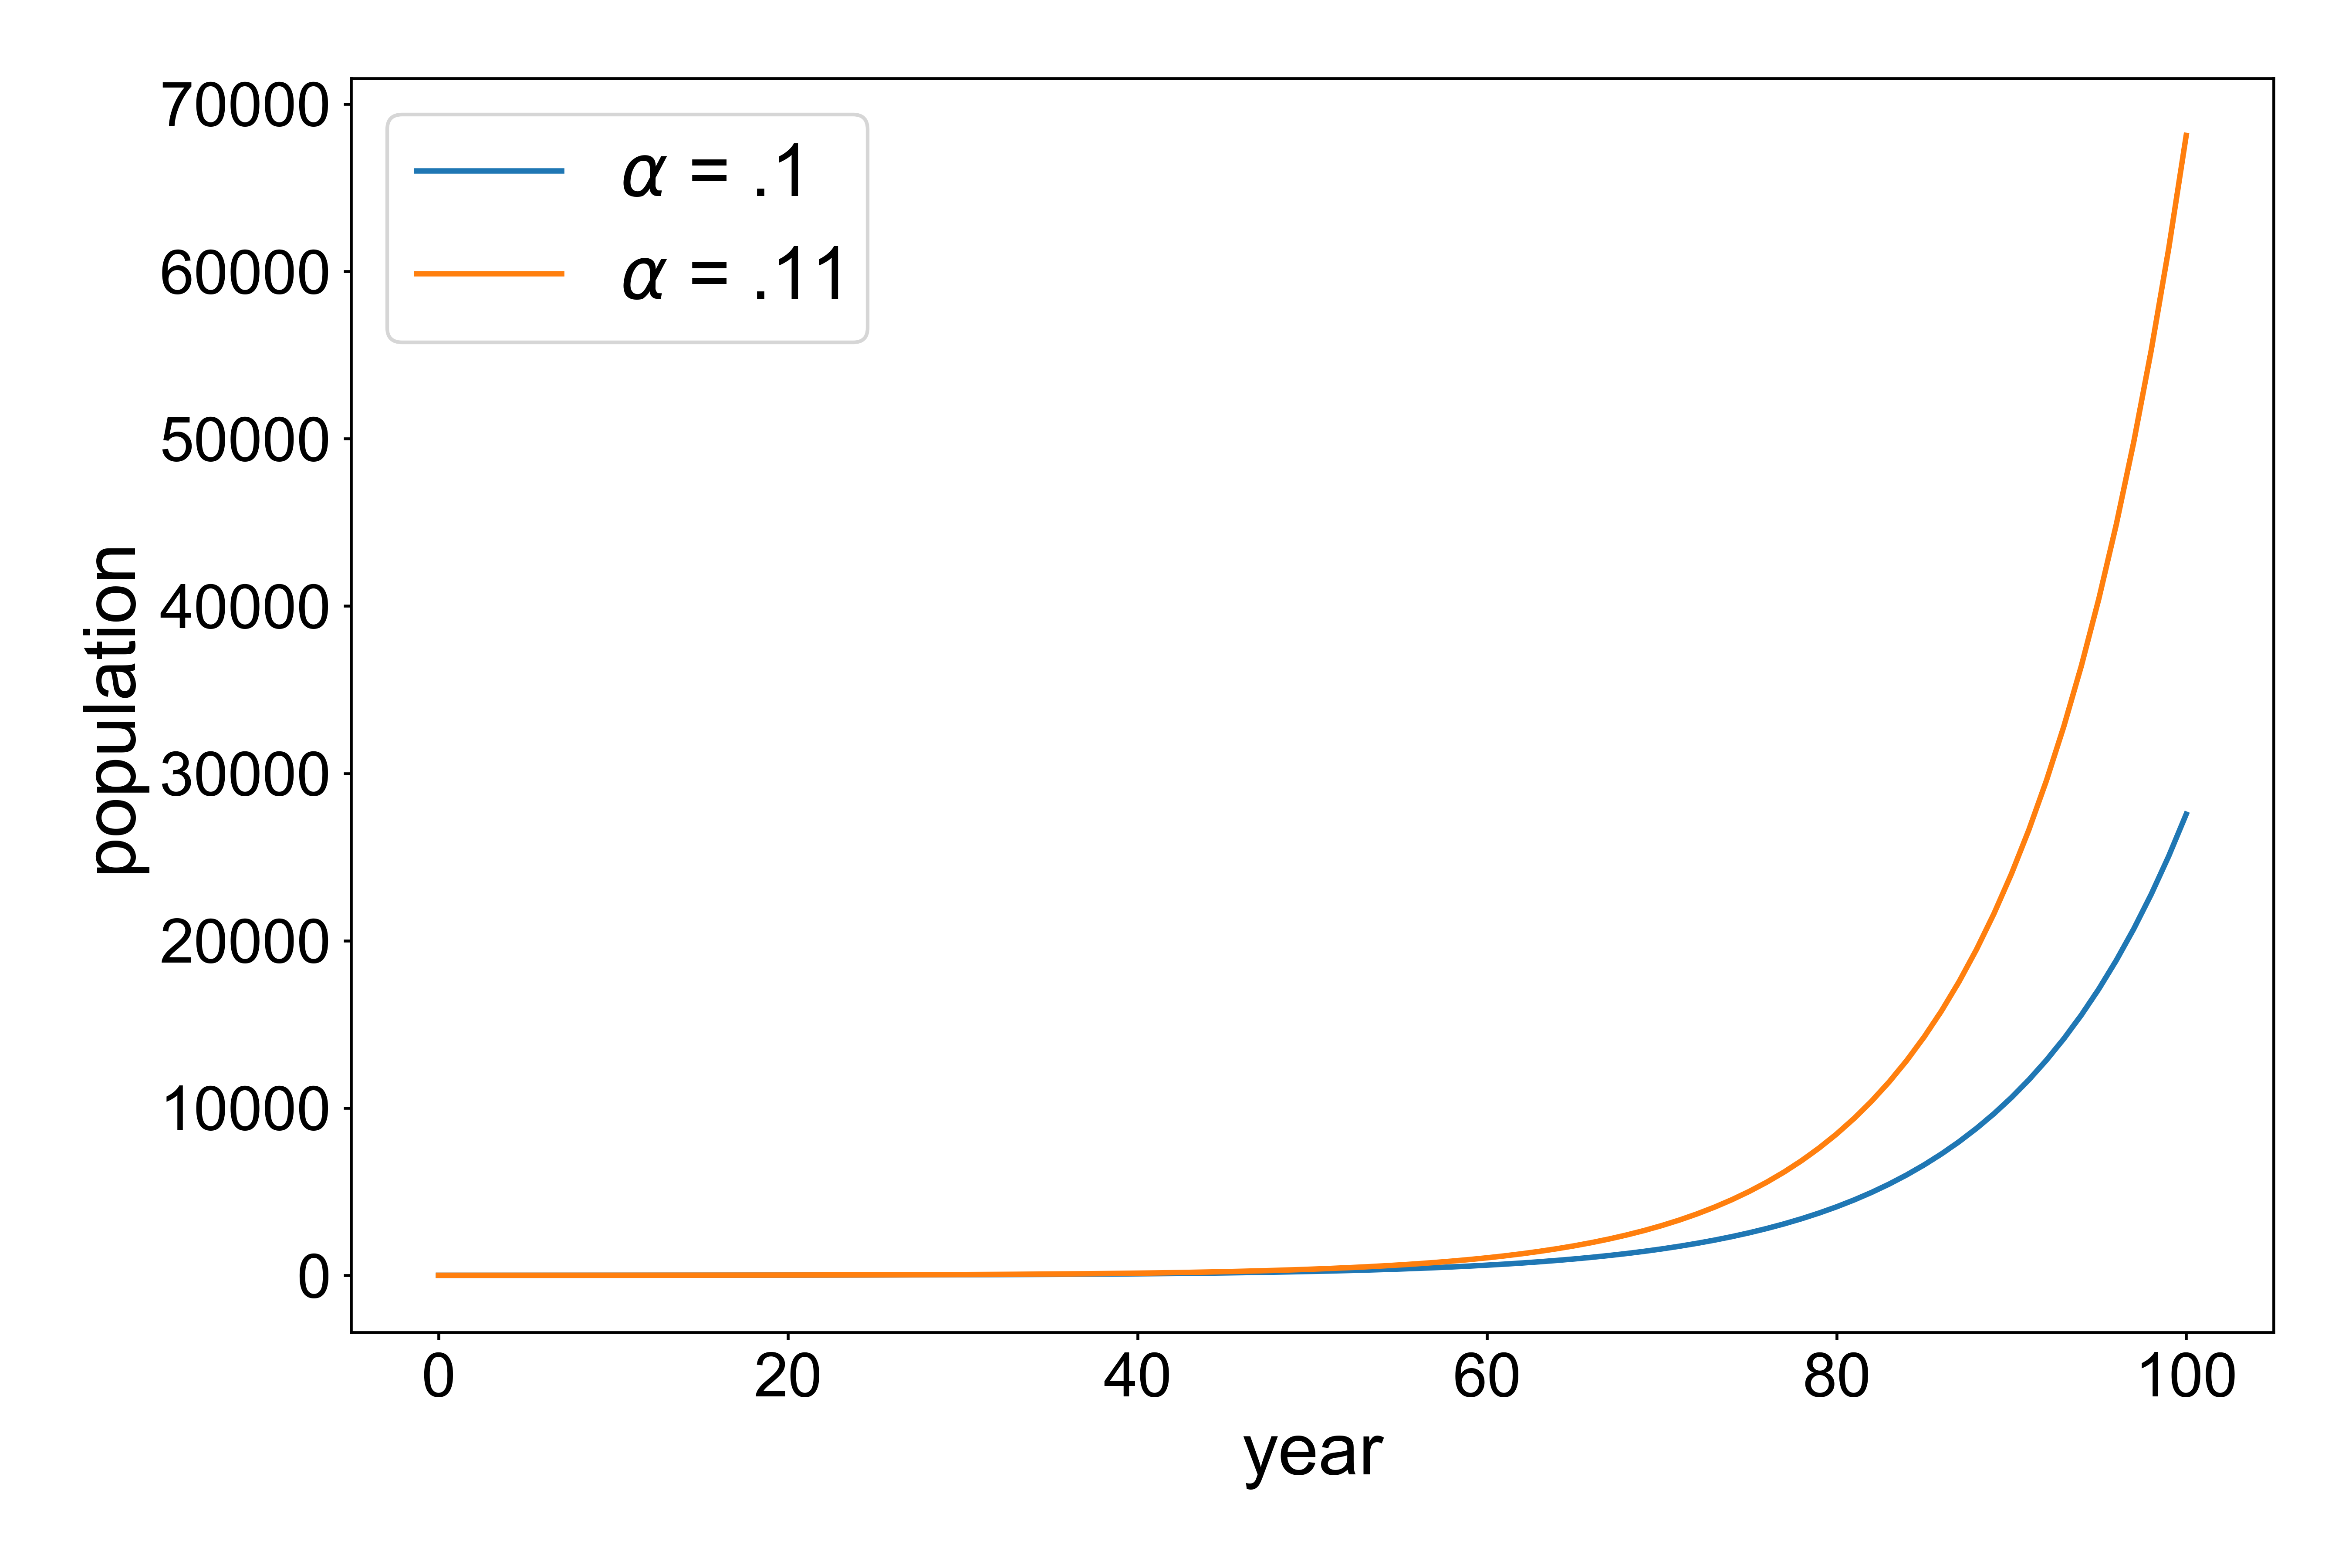
\includegraphics[width=1\linewidth]{fig1_report1.png}
     %\vspace*{-10.2mm}
  \end{subfigure}
  \begin{subfigure}[b]{.7\textwidth}
      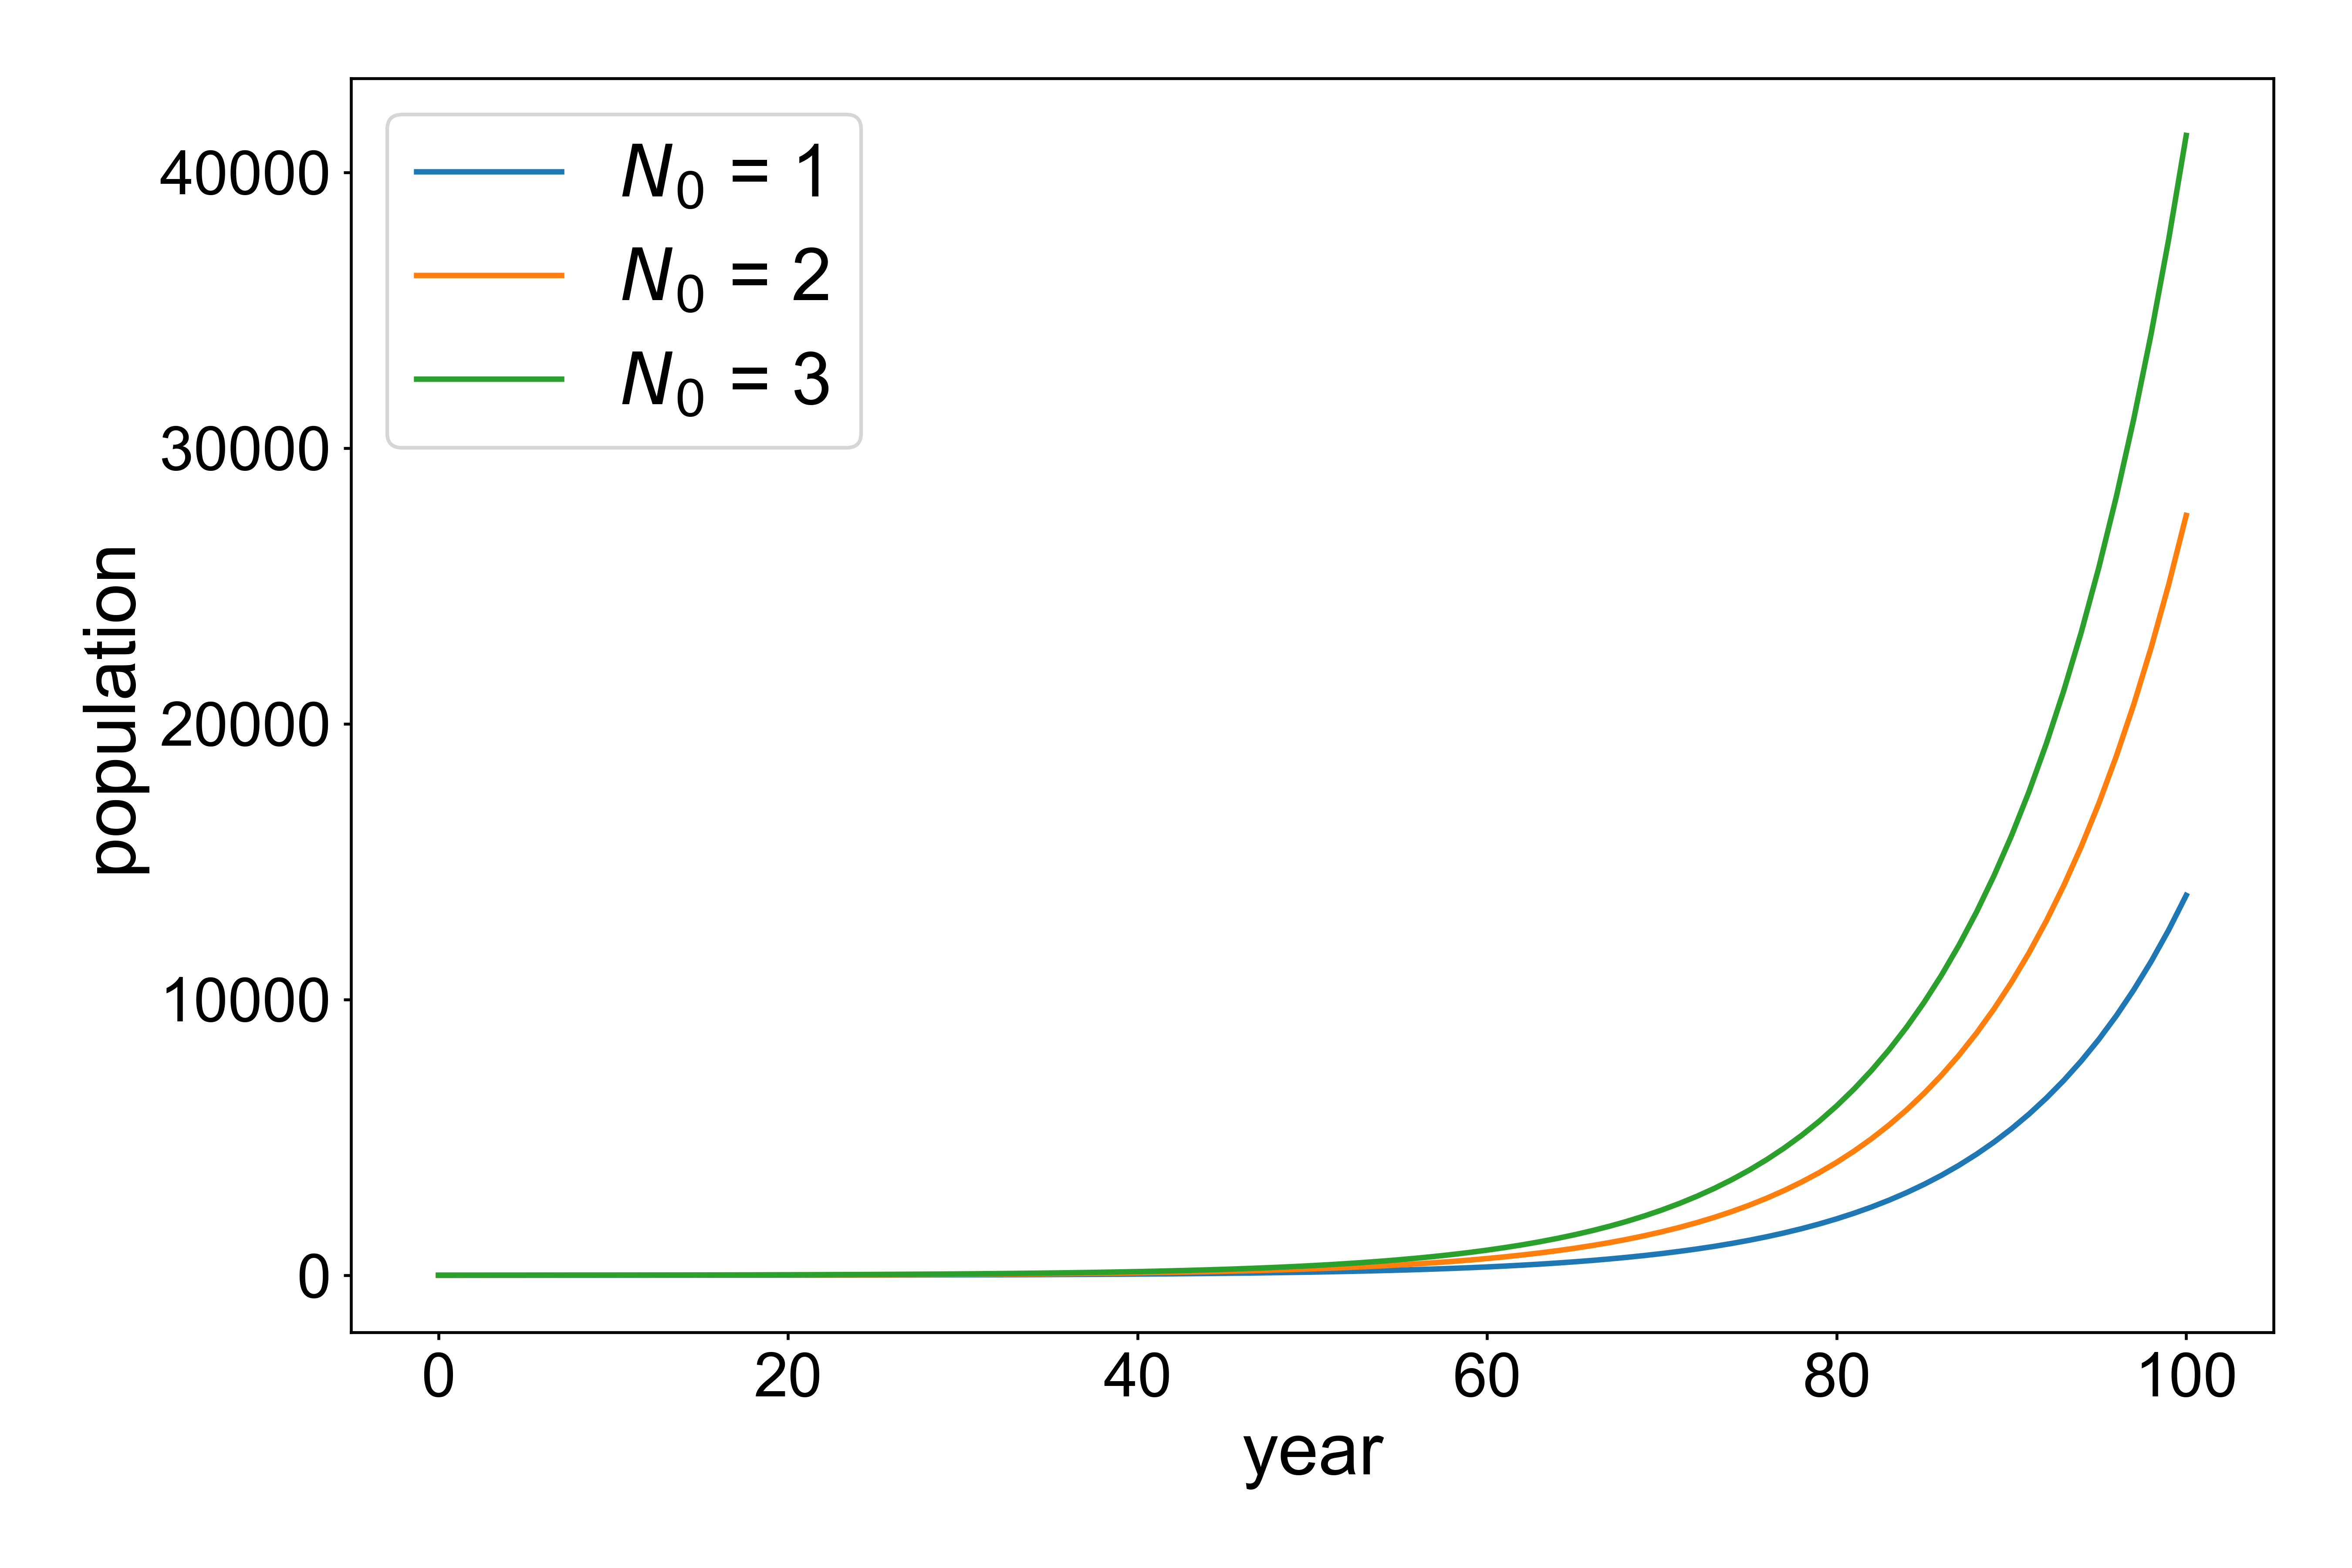
\includegraphics[width=1\linewidth]{fig1_report2.png}
      %\vspace*{-10.2mm}
   \end{subfigure}
  \caption[growing population]{\textbf{Top}. Population growth over a hundred years with a fixed $N_0 = 2$. \textbf{Bottom}. Same but with a fixed $\alpha = .1$}\label{fig:1stmod}
 \end{figure}



 %----------------------------------------------------------------------------------------
 %	SECTION 2
 %----------------------------------------------------------------------------------------
 \section{Modulating the growth}

 In the real world, there is indeed a finite amount of space and resources, and many other constraints that makes an exponential growth unplausible. Thus, we can consider that the more the population grows, the less spare resources there is. And consequently, the growth parameter depend on the current population. For instance, we can arbitrarily define \textit{$\alpha = 200 - p_{n-1}$}, with 200 thus being the maximal population possible for the environment, as the growth parameter $\alpha$ converge to 0 when the population converge to 200 (Figure \ref{fig:paramalpha}).




\begin{figure}[!htb]
\centering
  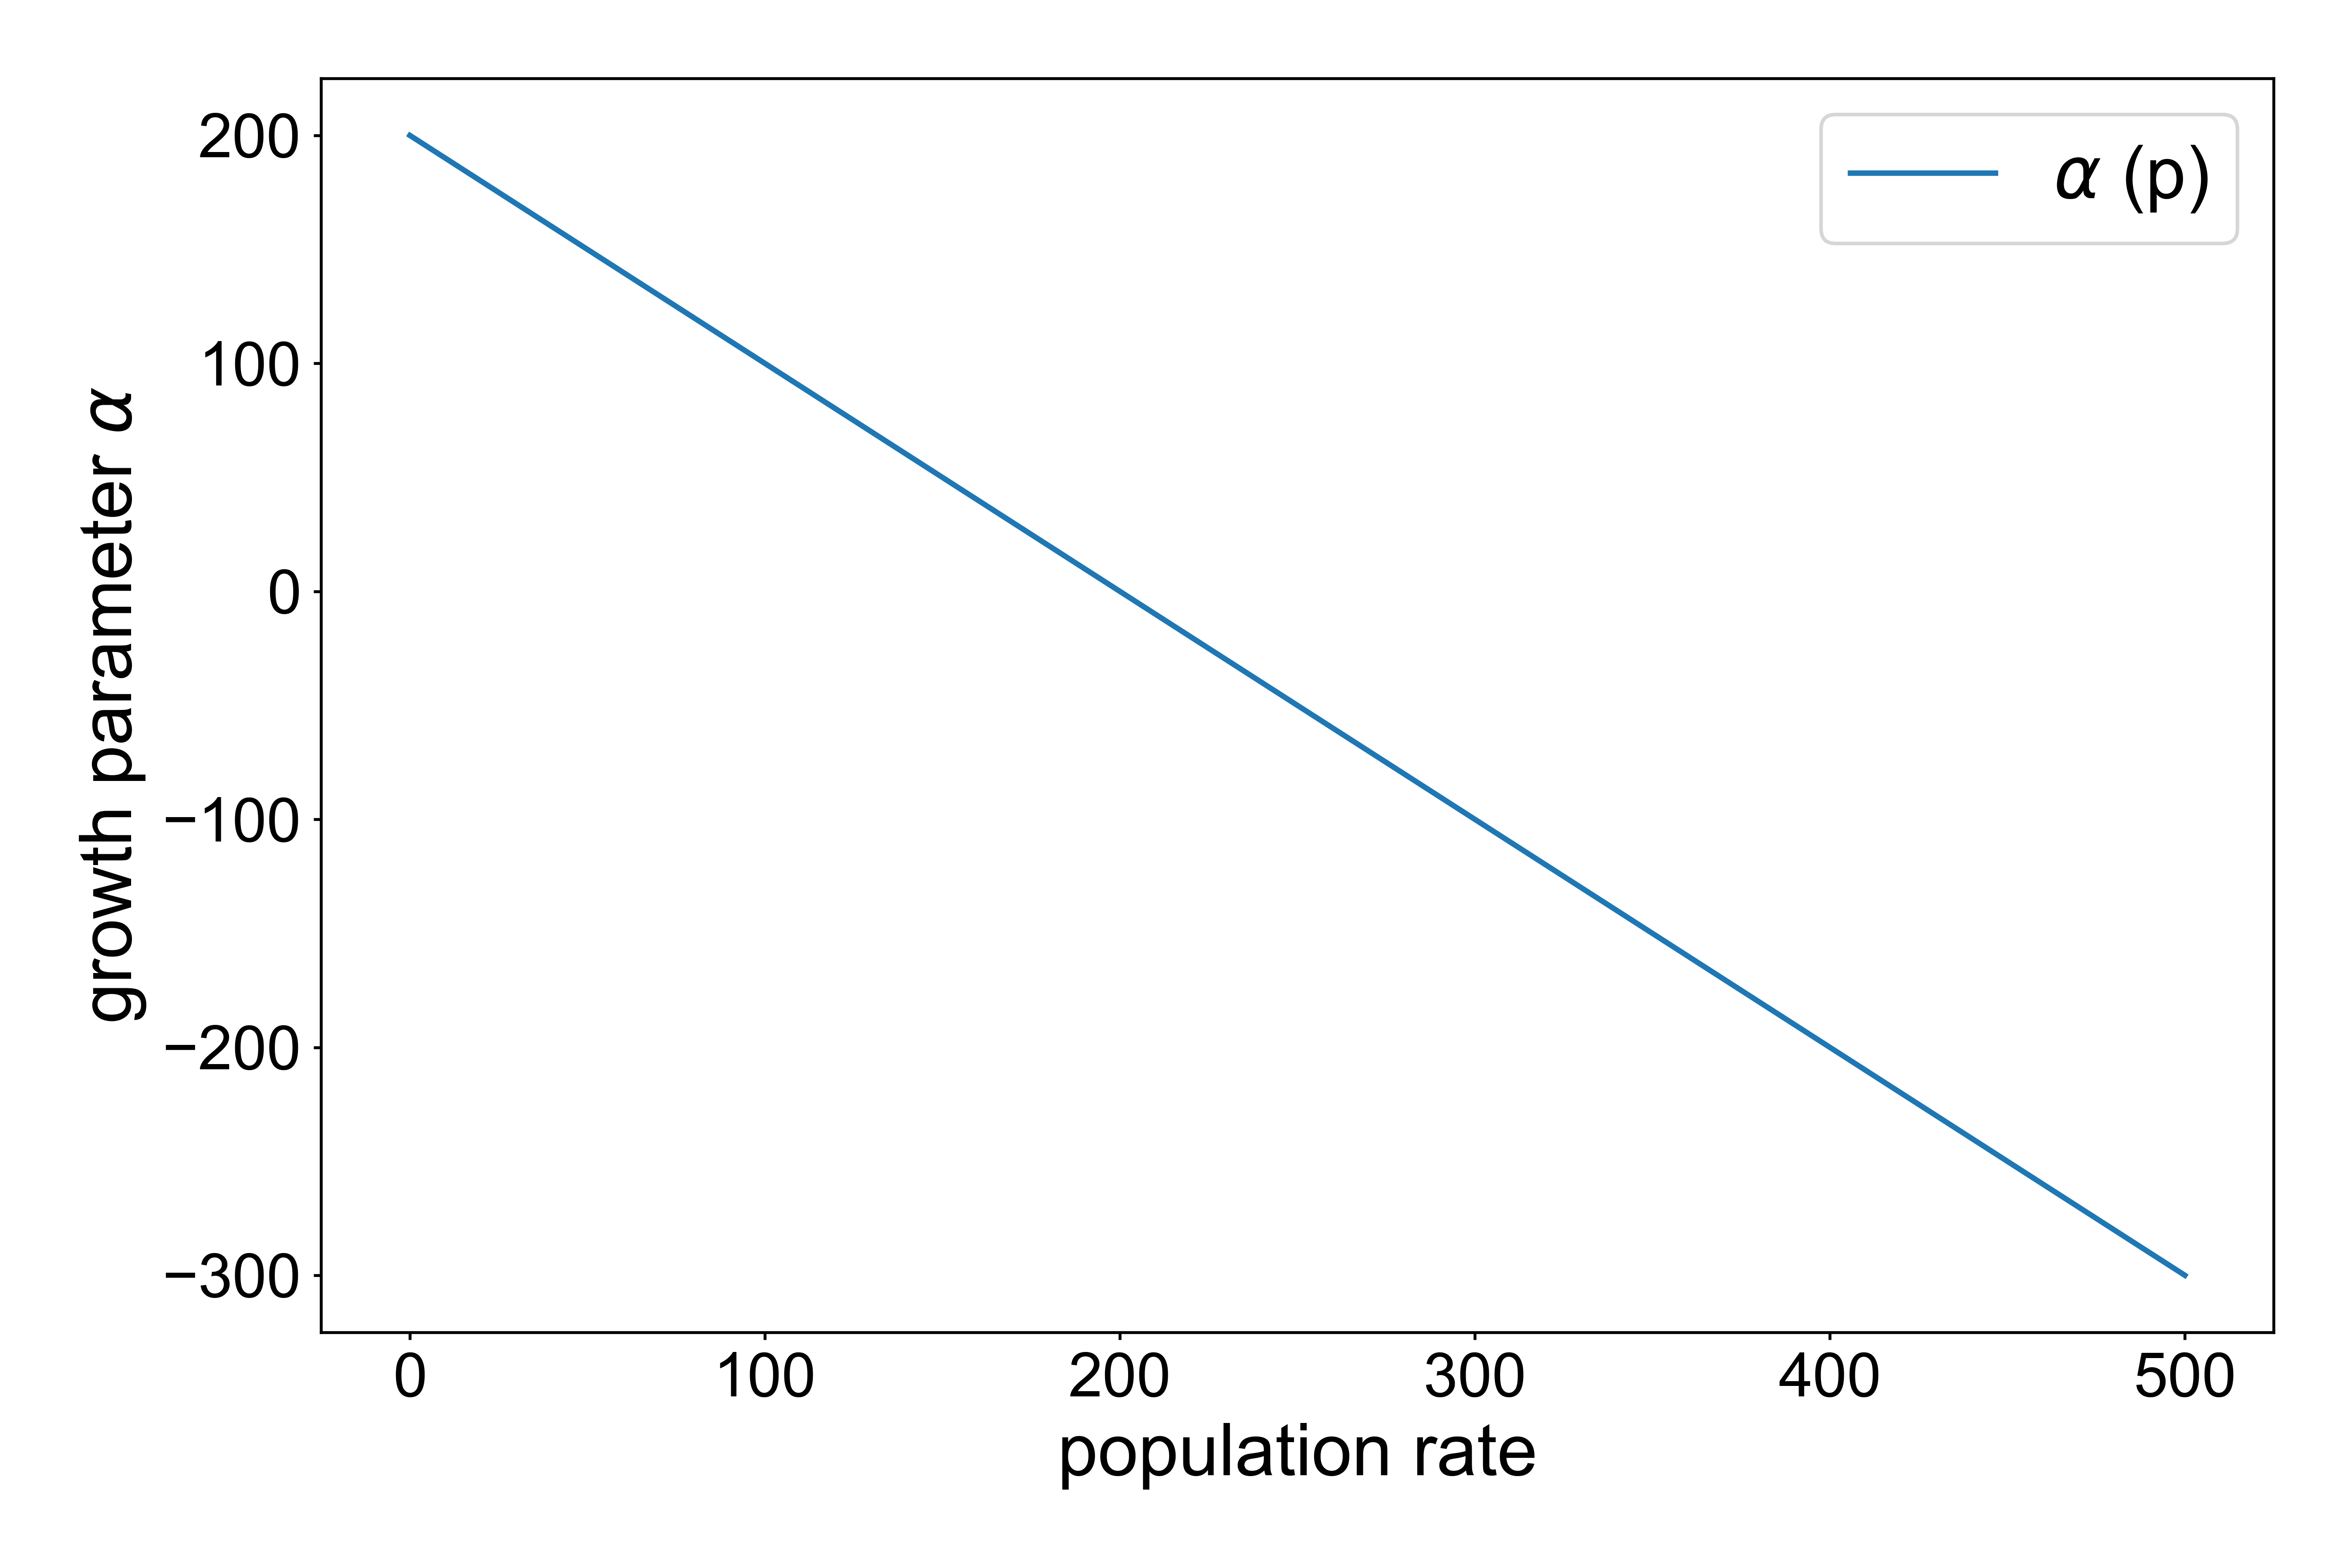
\includegraphics[width=.7\linewidth]{fig1_report3.png}
  \caption[population parameter] {Growth parameter $\alpha$ for a population between 1 and 500 individuals.}\label{fig:paramalpha}
\end{figure}



However, it seems we need to ``dilute" the new alpha coefficient, else if we start with $N_0 = 2$, the population the second year is going to be $2 + (200 -2) * 2 = 398$. So we would have overshot the $200$ threshold, and $\alpha$ becomes negative in the next year. This is good, but this model doesn't work anymore because alpha becomes to big, and this yields a population of $-1.6 * 10^{-5}$ on the third year.
If we introduce a small $\beta$ to diminish the influence of alpha, this growth becomes more progressive:

\begin{equation}\label{beta2}
p_n = p_{n-1} + \alpha \beta p_{n-1}
\end{equation}

Then if $\beta$ is small enough (\textit{$\beta$ <.01}), the growth is not too fast, and this yields a sigmoid curve (Figure \ref{fig:parambeta}). More precisely, the population undergoes a similar exponential growth at first, but then it slows down and reach a stationnary phase (when the population is 200).

\begin{figure}[!htb]
\centering
  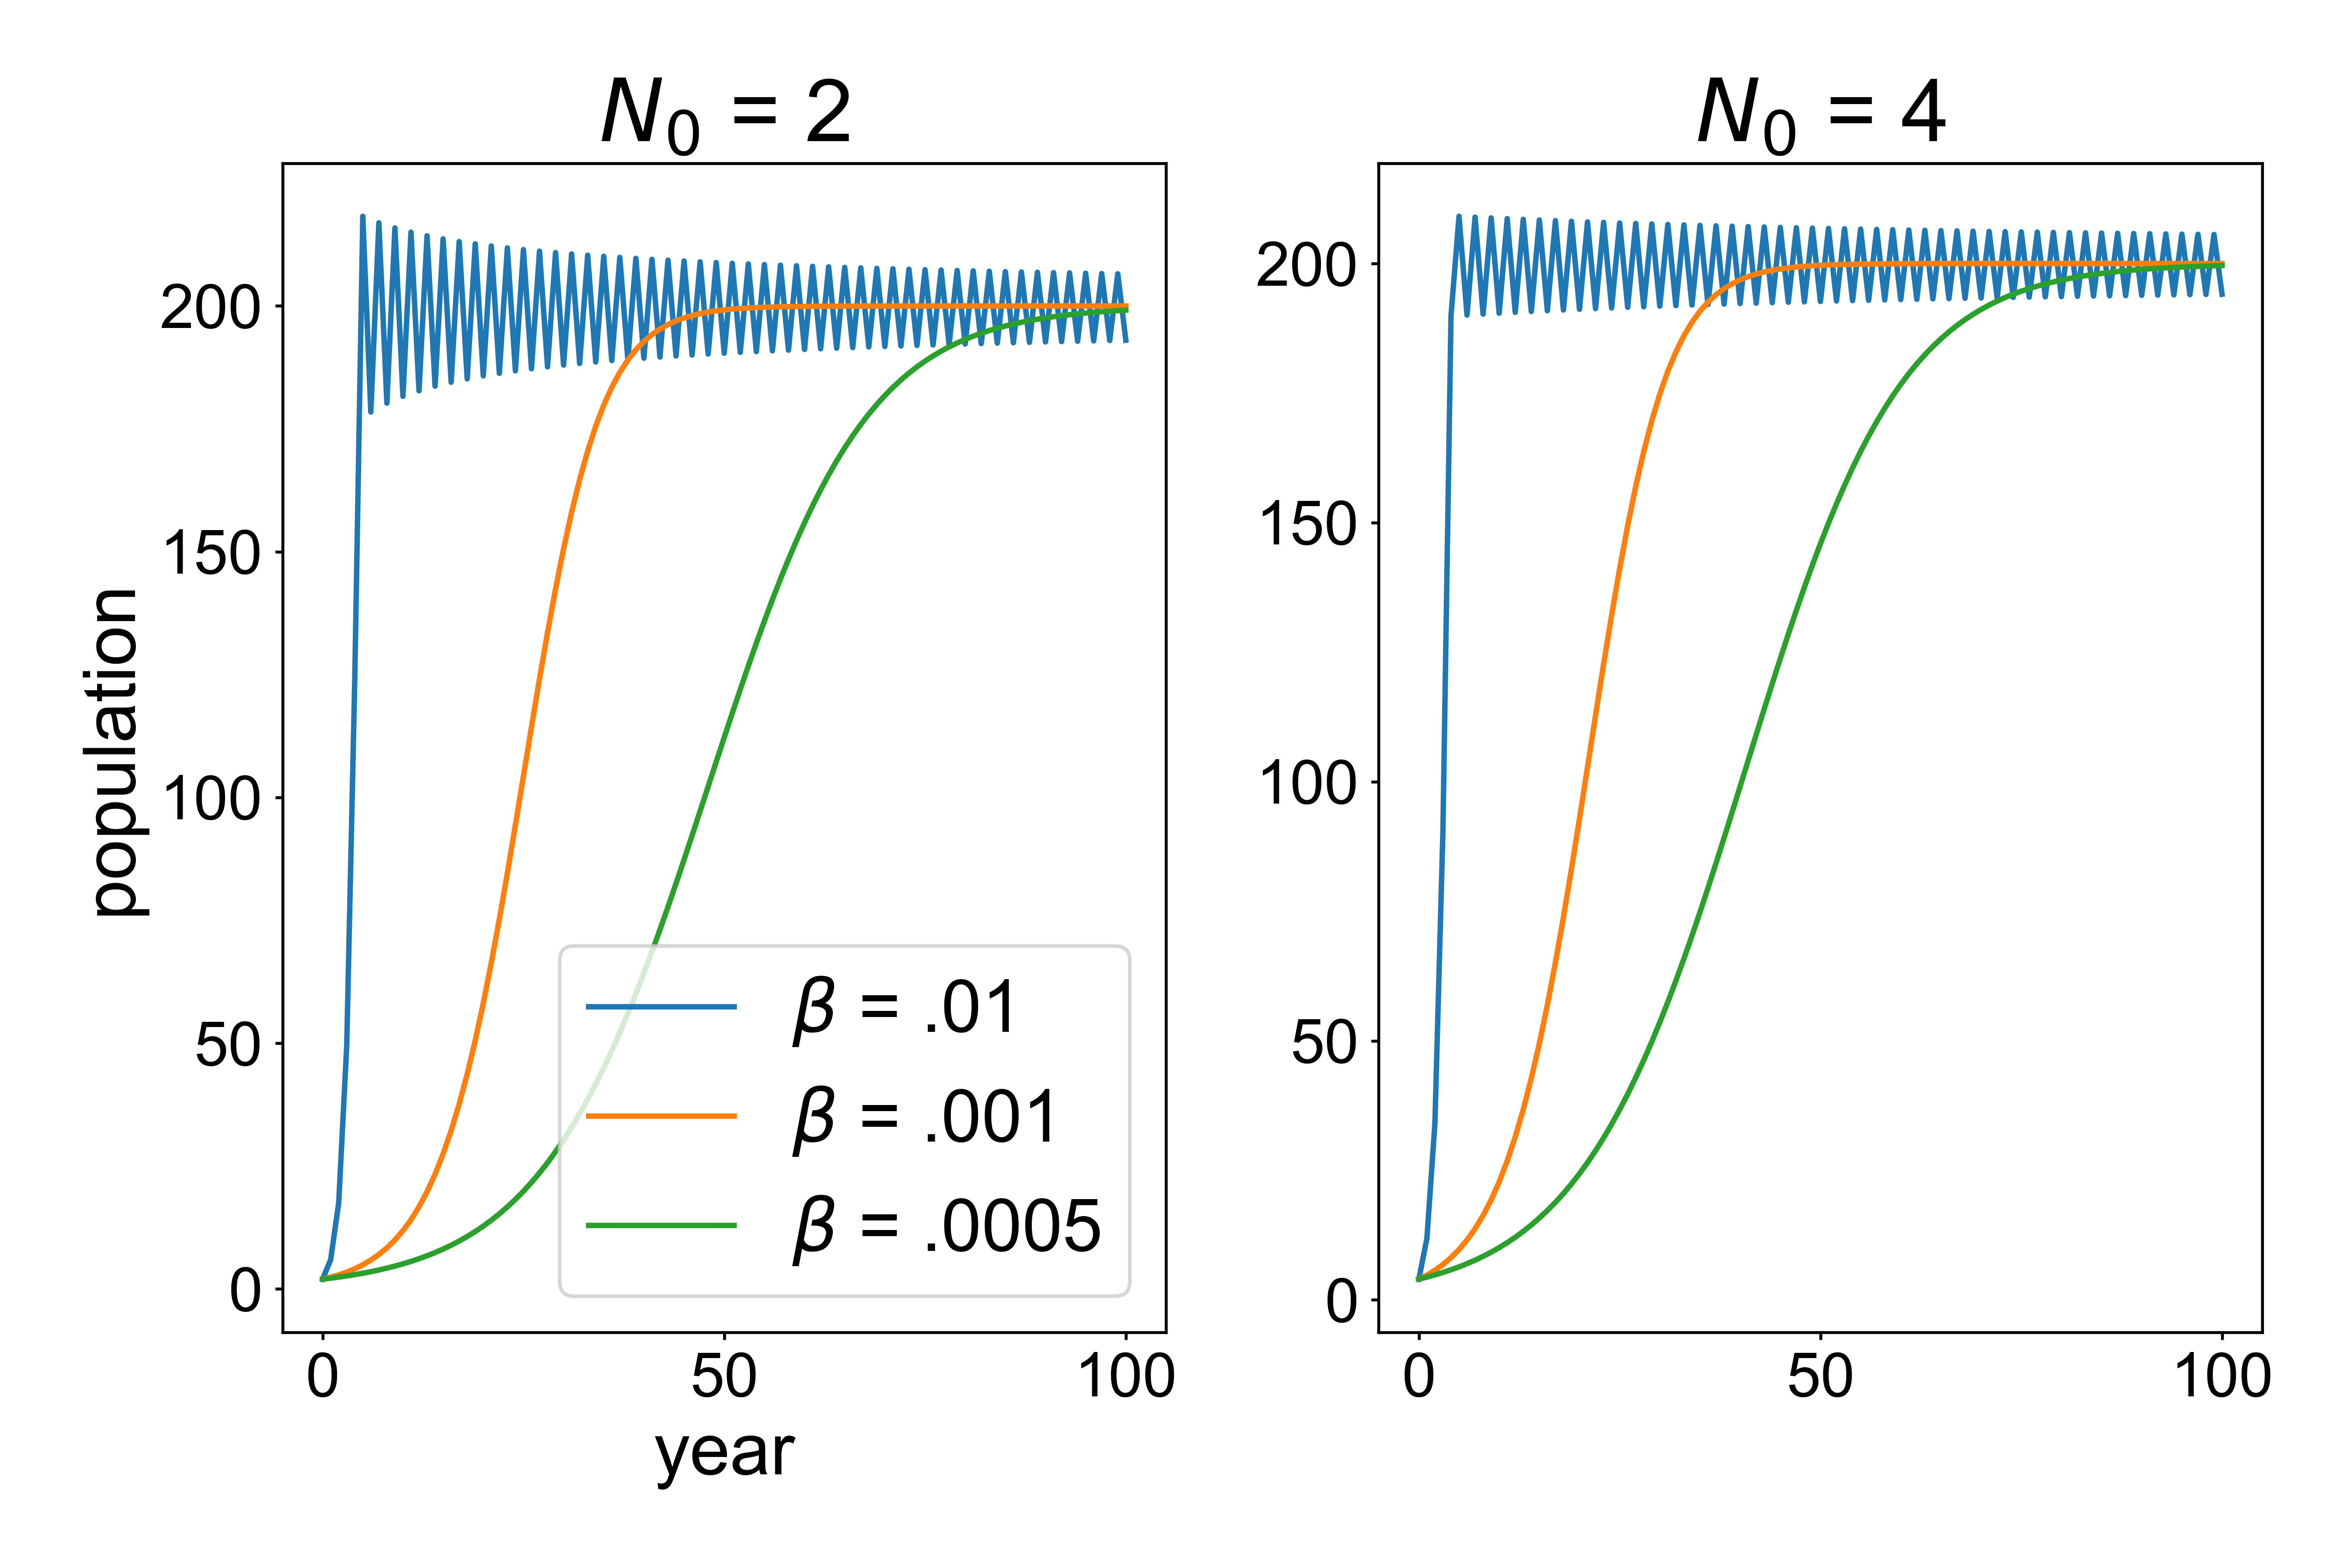
\includegraphics[width=1\linewidth]{fig1_report4.png}
  \caption[population parameter] {Different simulated growth for several $\beta$ parameters, with $N_0 = 2$ left and $N_0 = 4$ right pannel}\label{fig:parambeta}
\end{figure}

\end{document}
